\chapter{Постановка задачи и описание метода ее решения} 
\label{chapter2}

В данной главе обосновывается необходимость улучшения существующих подходов, описывается новый метод . TODO

\section{Задача}
SGM является оптимальным компромиссом качества и скорости по построению карт глубин на текущий момент. Для выполнения всех шагов алгоритма Semi-Global matching требуется $ O ( W \cdot H \cdot D) $ времени и $ O ( W *\cdot H * \cdot * D) $ памяти, где $W$ - ширина изображения, $H$ - высота изображения, $D$ - максимальная диспаратность. Ввиду того, что $D$ зависит от размера изображения, мы получаем нелинейное возрастание времени работы алгоритма от размера изображения. Несмотря на огромную разница в производительности относительно глобальных алгоритмов, время работы SGM на больших изображениях слишком велико и не сопоставимо со временем работы локальных алгоритмов. Качество, полученных результатов, близко к качеству глобальных алгоритмов. 
Поэтому попробуем изменить метод SGM для повышения скорости работы без потери качества.

\section{Метод с использованием приближенных вычислений.}

Качество любых алгоритмов построения карт глубин измеряется с помощью специальных пар картинок, для которых вручную созданы карты. Алгоритму подается такая пара изображений, затем по полученной с помощью него карте делается сравнение с эталонной. Для разных задач требуется разная точность диспаратностей, поэтому при измерении качества диспаратность пикселя считается верной, если она отличается не более, чем на определенную велечину. Алгоритмы могут давать хорошие результаты с большой погрешностью и плохие с маленькой. 

Предлагаемый метод получает на вход пару изображений, карту глубины с большой погрешностью и возвращает карту глубины с меньшей. Приближенную карту глубины мы можем посчитать с помощью быстрого, например локального, алгоритма, который строит карту с хорошим качеством при большой погрешности. 


Предлагаемый метод EA~+~RL основан на применении эволюционного алгоритма, настраиваемого во время выполнения с помощью обучения с подкреплением. Схема предлагаемого метода представлена на рис. \ref{ea-rl-scheme}. Красным цветом выделены особенности данной схемы, отличающие ее от схемы обучения с подкреплением, изображенной на рис. \ref{rl-scheme}. Агент взаимодействует со средой, ассоциируемой с ЭА. Он передает ФП, которая должна быть использована в следующем поколении с номером $t + 1$. Затем агент получает вознаграждение, зависящее от разности значений целевой ФП, вычисленной для лучших особей двух последних сгенерированных поколений. Он также получает состояние среды, зависящее от свойств текущего поколения. Генерируется новое поколение ЭА и процесс повторяется.

\begin{figure}[h!]
	\center{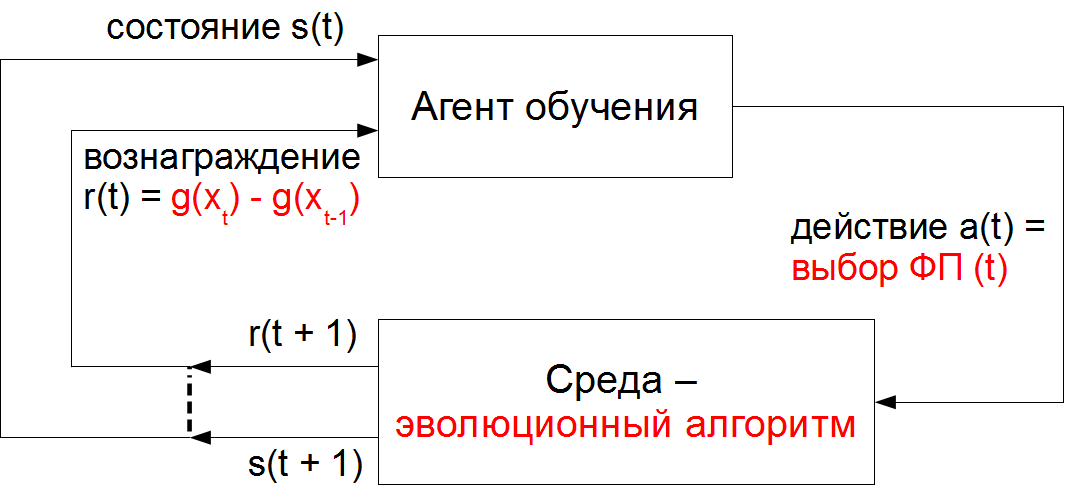
\includegraphics[width=0.6\textwidth]{ea-rl-scheme}}
	\caption{Схема предлагаемого метода}
	\label{ea-rl-scheme}
\end{figure}

Агент использует один из алгоритмов обучения с подкреплением, максимизирующий суммарное вознаграждение. Чем выше вознаграждение, тем, следовательно, значительнее был рост целевой ФП. Таким образом, оптимальный выбор ФП алгоритмом обучения ведет к лучшей производительности алгоритма оптимизации.

В следующих разделах приводится формальное представление задачи ускорения ЭА как задачи обучения с подкреплением, а также более детально описывается предлагаемый метод.

\subsection{Задача обучения с подкреплением}

Опишем имеющуюся задачу как задачу обучения с подкреплением~(\ref{rl}). Для этого достаточно задать множество действий агента $A$, способ определения состояний среды $s \in S$ и функцию вознаграждения $R : S \times A \rightarrow X \subseteq \mathbb{R}$. 

Будем обозначать особи, выращиваемые ЭА, как $x$. Пусть $G_i$ --- $i$-ое поколение. Множество действий $A$ соответствует множеству функций приспособленности, состоящему из $g$ --- целевой ФП и элементов множества $H$~--- вспомогательных ФП:
\begin{equation}\label{act}A = H \cup \{g\}.\end{equation}
Применение действия реализуется как выбор некоторой ФП $f_i \in A$ в качестве функции, используемой для оценки приспособленности особей ЭА, и формирования поколения $G_i$.


Введем обозначение для \emph{лучшей особи} поколения $G_i$, обладающей максимальным значением выбранной для этого поколения ФП $f_i$: 
$$z_i = \arg \max_{x \in G_i}{f_i(x)}.$$
Также введем обозначение для нормированной разности значений некоторой ФП, вычисленной на лучших особях двух последовательных поколений:
$$\Delta(f, i) = \frac{f(z_{i}) - f(z_{i - 1})} {f(z_{i})}, f \in A.$$

Каждому поколению ЭА поставим в соответствие состояние среды. Состояние $s_i$, соответствующее поколению $G_i$, представляет собой вектор функций приспособленности $f \in A$, упорядоченный по убыванию значений нормированных разностей $\Delta(f, i)$:
\begin{equation}\label{state}s_i = \langle f_1, f_2, \ldots f_{k + 1} \rangle: \Delta(f_1, i) \geq \Delta(f_2, i) \geq \ldots \Delta(f_{k + 1}, i).\end{equation}

В том случае, если для некоторых $f_a, f_b$ значение $\Delta(f_a, i)$ совпадает со значением $\Delta(f_b, i)$, функции $f_a, f_b$ располагаются в заранее установленном порядке. Например, пусть число вспомогательных ФП $k=2$ и в некотром поколении $G_i$ выполняется неравенство $\Delta(h_2, i) = \Delta(g, i) > \Delta(h_1, i)$. Тогда соответствующее состояние среды может иметь вид $s_i = \langle h_2, g, h_1 \rangle$ или $s_i = \langle g, h_2, h_1 \rangle$ в зависимости от начальной договоренности.

В заключение определим функцию вознаграждения $R : S \times A \rightarrow \{0, \frac{1}{2}, 1\}$, которая вычисляется после выбора действия $f_i$ в состоянии $s_{i-1}$ и генерации поколения $G_i$:
\begin{equation}
\label{reward}
 R(s_{i - 1}, f_i) =
  \begin{cases}
   1 & \text{если } g(z_{i}) - g(z_{i - 1}) > 0 \\
   \frac{1}{2} & \text{если } g(z_{i}) - g(z_{i - 1}) = 0 \\
   0 & \text{если } g(z_{i}) - g(z_{i - 1}) < 0 \\
  \end{cases}.
\end{equation}

Согласно (\ref{reward}), вознаграждение зависит от разности значений целевой ФП, посчитанной на лучших особях двух последовательных поколений. Значение вознаграждения наиболее высоко, когда целевая ФП растет. Напомним, что в обучении с подкреплением целью агента является максимизация суммарной награды, причем для ряда алгоритмов обучения с подкреплением доказана их сходимость к оптимальной стратегии поведения. Следовательно, задача обучения с подкреплением определена таким образом, что оптимальные действия агента будут приводить к максимизации прироста целевой ФП.

\subsection{Описание алгоритма EA~+~RL}

Предлагаемый метод позволяет управлять ходом выполнения эволюционного алгоритма путем назначения текущей ФП для каждого вновь сгенерированного поколения. Можно выделить две независимые сущности, составляющие основу метода: модуль обучения и эволюционный алгоритм. Будем называть эволюционный алгоритм средой обучения. Модулю обучения может быть передана награда и состояние среды. Он способен сообщать действие, которое необходимо применить к среде. В листинге \ref{rl-ga-method} представлен псевдокод разработанного алгоритма.
\begin{algorithm}[h!]
\caption{Метод оптимизации работы ЭА с помощью обучения}
\label{rl-ga-method}
%{\fontsize{12}{12}\selectfont
\begin{algorithmic}[1]
  \STATE {Инициализировать модуль обучения}
  \STATE {Установить номер текущего поколения: } $i \gets 0$
  \STATE {Сгенерировать начальное поколение } $G_0$
  \WHILE {(условие останова ЭА не выполнено)}
    \STATE {Вычислить состояние} $s_i$ {и передать его модулю обучения}
    \STATE {Получить ФП для следующего поколения } $f_{i+1}$ { из модуля обучения}
    \STATE {Сгенерировать следующее поколение} $G_{i+1}$
    \STATE {Вычислить вознаграждение: } $r \gets R(s_i, f_{i+1})$ { и передать его модулю обучения}
    \STATE {Обновить номер текущего поколения: } $i \gets i+1$
  \ENDWHILE
\end{algorithmic}
%}
\end{algorithm}
Модуль обучения может быть реализован на основе произвольного алгоритма обучения с подкреплением и взаимодействовать с произвольным эволюционным алгоритмом. В ходе выполнения работы было реализовано четыре различных алгоритма обучения: Q-learning \cite{sutton}, Delayed Q-learning \cite{delayed}, Dyna \cite{systems, survey} и R-learning \cite{r-learning}. Для обозначения различных реализаций предлагаемого метода EA~+~RL будем заменять в названии метода "EA" на название конкретного эволюционного алгоритма, "RL" --- на название алгоритма обучения с подкреплением. Например, если с помощью предлагаемого метода реализуется выбор ФП генетического алгоритма (ГА) c помощью алгоритма обучения Q-learning, то соответствующая реализация метода будет называться \emph{ГА~+~Q-learning}.

В качестве эволюционного алгоритма применялся генетический алгоритм \cite{mitchell-ga} с различными видами мутации и кроссовера. Также использовались различные виды эволюционных стратегий \cite{nature-inspired}. Эволюционные алгоритмы были реализованы на языке программирования \emph{Java} с помощью библиотеки эволюционных алгоритмов \emph{Watchmaker}~\cite{watchmaker}.

\section{Выводы по главе \protect\ref{chapter2}}
 Формализована цель исследований: разработка метода ускорения получения особей эволюционного алгоритма с высокими значениями целевой ФП при наличии конечного набора вспомогательных ФП. Описаны требования, предъявляемые к разрабатываемому методу. 
 Приведено сведение поставленной задачи к задаче обучения с подкреплением. Описан предлагаемый метод, основанный на назначении текущей ФП для каждого вновь сгенерированного поколения эволюционного алгоритма.
